% =========================================================================== %

\begin{frame}[t,plain]
\titlepage
\end{frame}

% =========================================================================== %

\begin{frame}[fragile]{e to the pi Minus pi}
%
\begin{center}
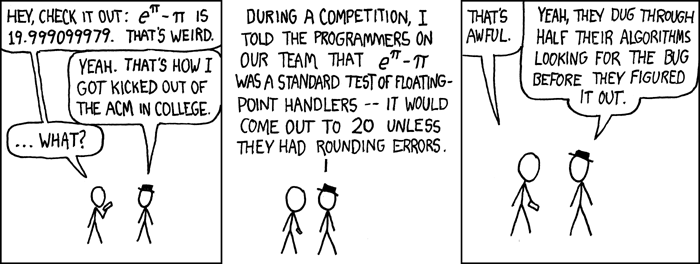
\includegraphics[width=.8\linewidth]{./gfx/18-xkcd-e_to_the_pi_minus_pi}

\vspace{12pt}
\emph{Also, I hear the 4th root of ($9^2 + {}^{19^2}/_{22}$) is pi.}

\vspace{6pt}
Source: \url{https://xkcd.com/217/}
\end{center}
%
\end{frame}

% =========================================================================== %

\begin{frame}{Scope For Today}
%
\begin{itemize}
\item Philosophy of testing
	\begin{itemize}
	\item Halting Problem
	\item Principal structure of test code
	\end{itemize}
\item Framework unittest
	\begin{itemize}
	\item Asserts
	\item Setup- and Teardown-Code
	\item Skipping Tests
	\end{itemize}
\item Mocking
	\begin{itemize}
	\item unittest.mock
	\item Return values and side effects
	\item Counting calls
	\end{itemize}
\item Notable mention: doctest
\end{itemize}
%
\end{frame}

% =========================================================================== %

\begin{frame}[fragile]{Formally Prooving Correctness}
%
\begin{itemize}
\item Programming is complex and it's easy to make mistakes$\phantom{.}^{\color{blue}\href{https://xkcd.com/285/}{\text{citation needed}}}$
\item Testing every possible input manually is tedious and equally prone to errors
\item[\Thus] It would be nice if we could simply proove correctness, \zB by means of a mathematical proof.
\pause
\item Not possible \emph{in general}
\item Possible for individual algorithms, of course ...
	\begin{itemize}
	\item There are proof assistants like \emph{Coq}\footnote{\texttt{https://coq.inria.fr/}}
	\end{itemize}
\item ... but not in the sense of: is the \emph{implementation} of the algorithm correct
\end{itemize}
%
\end{frame}

% =========================================================================== %

\begin{frame}{Example: Halting Problem}
%
\begin{itemize}
\item Given an arbitrary program $P$ with inputs $I$: does $P(I)$ halt?
	\begin{itemize}
	\item To halt: terminate, \ie not get stuck in an infinite loop
	\item You could extend the meaning to include \emph{without crashing} or \emph{and giving a desired output}
	\end{itemize}
\item Does a program $H: P, I \thus T$ exist?
	\begin{itemize}
	\item $T$: truth value, \ie boolean
	\end{itemize}
\pause
\item No, the problem is undecidable.
\item Proof by contradiction
	\begin{itemize}
	\item Assume $H$ with the above properties exists.
	\item Then we can construct a program $X$ that takes a program $Y$ as input:
		\begin{itemize}
		\item Run $T = H(Y, Y)$
		\item If $T == True$: go into infinite loop
		\item Otherwise, terminate.
		\end{itemize}
	\end{itemize}
\item[\Thus] What would $H(X, X)$ be?
\item[\Thus] Contradiction, undecidable problem
\end{itemize}
%
\end{frame}

% =========================================================================== %

\begin{frame}{Concept Unit Testing}
%
\begin{itemize}
\item Tests have to be specific to the problem and implementation at hand
\item Still, same form: \emph{extrinsic program} ($H$) that uses the \emph{code under test} ($P$)
\item The inputs $I$ to $P$ and the expected outputs $O$ must be provided by $H$
	\begin{itemize}
	\item Optimally: all conceivable combinations of inputs
	\item Usually just some representatives of normal and edge cases
		\begin{itemize}
		\item Exhaustive testing all $2^{64}$ values of one \inPy{float} input at 1\;ns per test: 585 years to complete
		\item Let alone storing all $2^{64}$ expected outputs
		\end{itemize}
	\item E.\;g.: Numbers: positive and negative, integers and decimal numbers, zero, infinity, epsilon
	\item Different Data Types
	\end{itemize}
\item[\Thus] $H$ calls as many routines of $P$ as possible, with as many variations of $I$ as reasonable
\end{itemize}
%
\end{frame}

% =========================================================================== %

\begin{frame}{Concept Unit Testing}
%
\begin{defbox}[Tweet by @brenankeller{,} Engineer at snapchat]
\small
A QA engineer walks into a bar. Orders a beer. Orders 0 beers. Orders 99999999999 beers. Orders a lizard. Orders -1 beers. Orders a ueicbksjdhd. 

\vspace{6pt}
First real customer walks in and asks where the bathroom is. The bar bursts into flames, killing everyone.
\begin{flushright}
\tiny
\url{https://twitter.com/brenankeller/status/1068615953989087232}
\end{flushright}
\end{defbox}
%
\begin{itemize}
\item[\Thus] There is no such thing as too much testing
\end{itemize}
%
\end{frame}

% =========================================================================== %

\begin{frame}[fragile]
%
\begin{codebox}[program.py]
\begin{minted}[fontsize=\scriptsize, linenos]{python3}
def add(x, y):
    return x + y
\end{minted}
\end{codebox}
%
\begin{codebox}[test.py]
\begin{minted}[fontsize=\scriptsize, linenos]{python3}
import program as cut  # code under test

inputs_and_expected_outputs = [((1, 1), 1), 
                               ((-1, 1), 0),
                               (("foo", "bar"), "foobar")]

for inputs, expected in inputs_and_expected_outputs:
    actual = cut.add(*inputs)
    if actual != expected:
        print("ERROR in method 'add' with inputs", inputs)
        print("  Expected:", expected)
        print("  Got     :", actual)
\end{minted}
\end{codebox}
%
\end{frame}

% =========================================================================== %

\begin{frame}{The Good, The Bad and the Ugly}
%
\begin{itemize}
\item Good
	\begin{itemize}
	\item Can be re-run as many times as we like, \ie whenever we make changes to our program
	\item Does not forget about relevant inputs
	\item Does not mix up lines from the lines of expected behaviours
	\item[\Thus] That's why it has become an industry standard
	\end{itemize}
\pause
\item Bad
	\begin{itemize}
	\item Tests need to be well-formed (correct) in the first place
	\item Provided set of inputs and expected outputs must cover the range of user inputs
	\item[\Thus] No way around, part of our job to be careful with tests
	\end{itemize}
\pause
\item Ugly
	\begin{itemize}
	\item This very simple framework forgets some important use cases
		\begin{itemize}
		\item We may want our program to \inPy{raise} exceptions
		\item Failing one test may or may not remove the need to run subsequent tests
		\end{itemize}
	\item It requires repetitive set-up code
		\begin{itemize}
		\item Constructing the same object-under-test such that it can be used with different inputs
		\end{itemize}
	\item[\Thus] Framework I'm about to show you
	\end{itemize}
\end{itemize}
%
\end{frame}

% =========================================================================== %

\begin{frame}{The \texttt{unittest} Framework}
%
\begin{itemize}
\item Set of classes and methods helping with common testing business
\item Usual steps
	\begin{itemize}
	\item \inPy{import unittest} -- pre-installed with Python
	\item Define a test fixture
		\begin{itemize}
		\item Simply a \inPy{class} derived from \texttt{unittest.TestCase}
		\item Should have one or several methods: \\
				Names begin with \texttt{test} \\
			 	Methods take only the \inPy{self} argument
		\item Each of them will be run once, without extra effort
		\item Usually calls special methods expressing the test intent \Thus \texttt{assert*} methods
		\item May have additional methods as needed
		\item Uses metaclass mechanism to register test cases
		\end{itemize}
	\item Call \texttt{unittest.main()}
		\begin{itemize}
		\item Usually done in a main module guard (\inPy{if __name__ == "__main__"})
		\item Usually in a separate main module (\texttt{project\_test.py})
		\end{itemize}
	\end{itemize}
\end{itemize}
%
\end{frame}

% =========================================================================== %

\begin{frame}[fragile]
%
\vspace{-9pt}
\begin{tcbraster}[raster columns=2,
                  raster equal height,
                  nobeforeafter,
                  raster column skip=0.1cm]
\begin{codebox}[testFoo.py]
\begin{minted}[fontsize=\scriptsize,linenos]{python3}
import program as cut
import unittest

class TestClassFoo(unittest.TestCase):
    def test_default_state(self):
        """Well defined default state"""
        foo = cut.Foo()
        self.assertTrue(foo.is_ready())
        self.assertFalse(foo.is_active())
        self.assertEqual(
            foo.get_listener_count(), 0)

    def test_raises_errors(self):
        foo = cut.Foo()
        self.assertRaisesRegex(
            foo.run(),
            "not active", 
            cut.StateError)

if __name__ == "__main__":
    unittest.main()
\end{minted}
\end{codebox}
%
%\vspace{-12pt}
\begin{cmdbox}[Output]
\begin{minted}[fontsize=\scriptsize]{text}
==========================================
FAIL: test_default_state (__main__
    .TestClassFoo
    .test_default_state)
Well defined default state
------------------------------------------
Traceback (most recent call last):
  File "testFoo.py", line 8, in 
      test_default_state
    self.assertTrue(foo.is_ready())
    ^^^^^^^^^^^^^^^^^^^^^^^^^^^^^^^
AssertionError: foo.is_ready() is not true
\end{minted}
\end{cmdbox}
\end{tcbraster}
%
\end{frame}

% =========================================================================== %

\begin{frame}{Benefits Over Minimal Framework So Far}
%
\begin{itemize}
\item Helpful error messages
	\begin{itemize}
	\item 33 specialized \texttt{assert*} methods
	\end{itemize}
\item Ability to handle exceptions
	\begin{itemize}
	\item React to both, error class and text
	\end{itemize}
\item All tests started with one single line
\item Grouping of tests into multiple fixtures according to theme/tested unit
\item Interactions with IDEs
	\begin{itemize}
	\item Often special views for test results
	\end{itemize}
\end{itemize}
%
\end{frame}

% =========================================================================== %

\begin{frame}{Asserts -- Generic}
%
\rowcolors{2}{tabhighlight}{white}
\scriptsize
%
\begin{tabular}{llm{.4\linewidth}}
\textbf{Method} & \textbf{Checks That} & \textbf{Remarks} \tabcrlf

\texttt{assertTrue(x)}              & \inPy{bool(x) is True} &
	\multirow{2}{\linewidth}{In principle enough to formulate all tests} \\
\texttt{assertFalse(x)}             & \inPy{bool(x) is False} \tabcrlf

\texttt{assertIsNone(x)}            & \inPy{x is None} \\
\texttt{assertIsNotNone(x)}         & \inPy{x is not None} \tabcrlf

\texttt{assertEqual(a, b)}          & \texttt{a == b} & 
	\multirow{2}{\linewidth}{\texttt{addTypeEqualityFunc} can be used to register compare functions}
	\\
\texttt{assertNotEqual(a, b)}       & \inPy{a != b} \tabcrlf

\texttt{assertIs(a, b)}             & \inPy{a is b} \\
\texttt{assertIsNot(a, b)}          & \inPy{a is not b} \tabcrlf

\texttt{assertIsInstance(a, b)}     & \inPy{isinstance(a, b)} &
	\multirow{2}{\linewidth}{\texttt{b} must be a \inPy{class}} \\
\texttt{assertNotIsInstance(a, b)}  & \inPy{not isinstance(a, b)} \tabcrlf
\end{tabular}
%
\end{frame}

% =========================================================================== %

\begin{frame}{Asserts -- Numbers}
%
\rowcolors{2}{tabhighlight}{white}
\scriptsize
\begin{tabular}{lm{.2\linewidth}m{.4\linewidth}}
\textbf{Method} & \textbf{Checks That} & \textbf{Remarks} \tabcrlf
\texttt{assertAlmostEqual(a, b)}    & \inPy{round(a-b, 7) == 0} & 
	\multirow{2}{\linewidth}{Additional Parameters \texttt{places} (decimal places) or \texttt{delta} (absolute difference)}
	\\
\texttt{assertNotAlmostEqual(a, b)} & \inPy{round(a-b, 7) != 0} \tabcrlf
\texttt{assertGreater(a, b)}        & \inPy{a > b} \\
\texttt{assertGreaterEqual(a, b)}   & \inPy{a >= b} \\
\texttt{assertLess(a, b)}           & \inPy{a < b} \\
\texttt{assertLessEqual(a, b)}      & \inPy{a <= b} \tabcrlf
\end{tabular}
%
\begin{hintbox}[Equality of \texttt{float}s]
\footnotesize
For \inPy{float}s \texttt{a} and \texttt{b}, the expression \texttt{a == b} \emph{is} well-defined, but usually not what we want. Due to inevitable rounding errors baked into floating point logic, we alwas need to provide a tolerance range.

\vspace{3pt}
Try \inPy{print(0.1 + 0.1 + 0.1)}
\end{hintbox}
%
\end{frame}

% =========================================================================== %

\begin{frame}{Asserts -- Strings and Collections}
%
\rowcolors{2}{tabhighlight}{white}
\scriptsize
\begin{tabular}{lm{.2\linewidth}m{.4\linewidth}}
\textbf{Method} & \textbf{Checks That} & \textbf{Remarks} \tabcrlf
\texttt{assertRegex(s, r)}          & \inPy{r.search(s)} &
	\multirow{2}{\linewidth}{
		We'll cover Regexes in detail soon.\\
		For now, read as \enquote{\texttt{s} contains \texttt{r}}}
	\\
\texttt{assertNotRegex(s, r)}       & \inPy{not r.search(s)} \tabcrlf
\texttt{assertIn(a, b)}             & \inPy{a in b} & 
	\multirow{2}{\linewidth}{\inPy{type(b)} must implement \inPy{__contains__}} \\
\texttt{assertNotIn(a, b)}          & \inPy{a not in b} \tabcrlf
\texttt{assertCountEqual(a, b)}     & &
	\texttt{a} and \texttt{b} have the same elements in the same number, regardless of their order.
	\tabcrlf
\texttt{assertMultiLineEqual(a, b)} & & compares \inPy{str}ings \\
\texttt{assertSequenceEqual(a, b)}  & & compares sequences \\
\texttt{assertListEqual(a, b)}      & & compares \inPy{list}s \\
\texttt{assertTupleEqual(a, b)}     & & compares \inPy{tuple}s \\
\texttt{assertSetEqual(a, b)}       & & compares \inPy{set}s or \inPy{frozenset}s \\
\texttt{assertDictEqual(a, b)}      & & compares \inPy{dict}s \\
\end{tabular}
%
\end{frame}

% =========================================================================== %

\begin{frame}{Asserts -- Errors}
%
\rowcolors{2}{tabhighlight}{white}
\scriptsize
\begin{tabular}{lm{.4\linewidth}}
\textbf{Method} & \textbf{Checks That} \tabcrlf

\texttt{assertRaises(exc, fun, *args, **kwds)} &
	\texttt{fun(*args, **kwds)} raises \texttt{exc} \\

\texttt{assertRaisesRegex(exc, r, fun, *args, **kwds)} &
	\texttt{fun(*args, **kwds)} raises \texttt{exc} and the message matches regex \texttt{r} 
	\tabcrlf

\texttt{assertWarns(warn, fun, *args, **kwds)} &
	\texttt{fun(*args, **kwds)} raises \texttt{warn} \\

\texttt{assertWarnsRegex(warn, r, fun, *args, **kwds)} &
	\texttt{fun(*args, **kwds)} raises \texttt{warn} and the message matches regex \texttt{r}
	\tabcrlf

\texttt{assertLogs(logger, level)} &
	The \texttt{with} block logs on logger with minimum level \\

\texttt{assertNoLogs(logger, level)} &
	The with block does not log on logger with minimum level
\end{tabular}
%
\begin{hintbox}[Warnings and Log Messages]
\footnotesize
The modules \href{https://docs.python.org/3/library/warnings.html}{\thus \texttt{warnings}} and \href{https://docs.python.org/3/library/logging.html}{\thus \texttt{logging}} provide utilities for professional-looking messages to users and devellopers. The \texttt{assertWarns*} and \texttt{assert*Logs} methods react to these utilities.
\end{hintbox}
%
\end{frame}

% =========================================================================== %

\begin{frame}[fragile]{Tangent: Testing Guidelines (1): Scope of a Test}
%
\begin{itemize}
\item Avoid too many dependent lines of code
	\begin{itemize}
	\item 
		\begin{minted}{python3}
foo.set_property_1(None)
self.assertTrue(foo.property_1_is_good())
foo.set_property_2(None)
self.assertTrue(foo.property_2_is_good())
		\end{minted}
	\item Does \texttt{property\_2} depend on \texttt{property\_1}?
	\item First assert may hide failure of second assert
	\end{itemize}
\item Rather write several small test cases
\item SRP also applies to tests!
\pause
\item[\Thus] It would be nice to have a way to automate setup- and teardown code
\end{itemize}
%
\end{frame}

% =========================================================================== %

\begin{frame}{Automating Setup- and Teardown-Code}
%
\begin{itemize}
\item Method \inPy{setUp(self)}
	\begin{itemize}
	\item If defined, automatically called before each \texttt{test*} method
	\item May define instance attributes of the class (\inPy{self.foo = Foo(*default_attributes)})
	\end{itemize}
\item Likewise: Method \inPy{tearDown(self)}
	\begin{itemize}
	\item Automatically called after each \texttt{test*} method (if present at all)
	\item Used for cleanup work like closing and removing files, disconnecting from servers, ...
	\end{itemize}
\pause
\item Similar: \inPy{setUpClass(cls)} and \inPy{tearDownClass}
	\begin{itemize}
	\item Called automatically once per test suite
	\item Must be decorated with \inPy{@classmethod}
	\item \inPy{cls} instead of \inPy{self} -- sets class attributes rather than instance attributes
	\item Often used to set up a specific directory structure
	\end{itemize}
\end{itemize}
%
\end{frame}

% =========================================================================== %

\begin{frame}[fragile]
%
\vspace{-12pt}
\begin{codebox}[testFoo.py]
\begin{minted}[fontsize=\scriptsize,linenos]{python3}
import unittest
import tempfile
import pathlib

class TestClassFoo(unittest.TestCase):
    @classmethod
    def setUpClass(cls):        # called once
        cls.data_directory = pathlib.Path(tempfile.gettempdir()) / "FooTest"
        cls.data_directory.mkdir()
    
    @classmethod
    def tearDownClass(cls):     # called once
        cls.data_directory.rmdir()
        
    def setUp(self):            # called multiple times
        restore_default_files(self.data_directory)
    
    def tearDown(self):         # called multiple times
        make_empty_directory(self.data_directory)
    
    def test_1(self):
        ...
\end{minted}
\end{codebox}
%
\end{frame}

% =========================================================================== %

\begin{frame}{Tangent: Testing Guidelines (2): Directory Structure}
%
\begin{itemize}
\item Usually: 2..4 directories: \texttt{src} (productive code), \texttt{src-test} (test code),\\
	\texttt{res} (files needed by productive code), \texttt{res-test} (files needed by test)
\item Access to \texttt{res-test} should be read-only
	\begin{itemize}
	\item Test must always be in a well-defined state
	\item Accidental changes by a mal-formed program may render a test \emph{flaky} and generally hard to debug (bug in Code or test?)
	\item[\Thus] If write-access needed for test: copy from \texttt{src-test} to a temp-dir
	\end{itemize}
\end{itemize}
%
\begin{hintbox}[Lingu: Flaky Tests]
\footnotesize
Flaky code is code that seems to work sometimes but not everytime, even though the code has not changed between executions.
Reasons are often external dependencies or timing issues in multithreaded algorithms.
\end{hintbox}
%
\end{frame}

% =========================================================================== %

\begin{frame}{Skipping Tests}
%
\begin{itemize}
\item Sometimes: Tests not applicable in some situations
	\begin{itemize}
	\item OS-Specific code
	\item Version of dependencies
	\item Known bug, but focus devellopment on other aspects
	\end{itemize}
\item (Conditional) skipping of tests
\item Method \texttt{unittest.skipTest(reason\_string)}
\item Decorator \texttt{unittest.skip(reason)}, \texttt{skipIf(condition, reason)} and \texttt{skipUnless(condition, reason)}
\end{itemize}
%
\begin{hintbox}[Avoid Unconditional Skips]
\footnotesize
Even when focussing on other issues, use the condition \emph{current date < deadline} to avoid forgetting about the issue.
\end{hintbox}
%
\end{frame}

% =========================================================================== %\\

\begin{frame}[fragile]
%
\begin{codebox}[skipTests.py]
\begin{minted}[fontsize=\scriptsize,linenos]{python3}
class MyTestCase(unittest.TestCase):

    @unittest.skip("demonstrating skipping")
    def test_nothing(self):
        self.fail("shouldn't happen")

    @unittest.skipIf(mylib.__version__ < (1, 3), "not supported in this library version")
    def test_format(self):
        ...

    @unittest.skipUnless(sys.platform.startswith("win"), "requires Windows")
    def test_windows_support(self):
        ...

    def test_maybe_skipped(self):
        if not external_resource_available():
            self.skipTest("external resource not available")
        ...
\end{minted}
\end{codebox}
%
\end{frame}

% =========================================================================== %

\begin{frame}{Mocking}
%
\begin{itemize}
\item Common Problem: Dependency on other structures
	\begin{itemize}
	\item Example: We need to test the \emph{strubling} behaviour of the \texttt{FeebleStrubler}\footnote%
		{Of course, \emph{Feeble}, \emph{to struble} and \emph{Flobox} are fantasy words here}
	\item The \texttt{FeebleStrubler} needs one or more \texttt{Feeble}s to work on
	\item A \texttt{Feeble} is an aggregate of several \texttt{Flobox}es
	\item All of them are nontrivial to set up and/or require considerable system ressources/runtime
	\end{itemize}
\pause
\item[\Thus] Desire to \emph{mock} these components
	\begin{itemize}
	\item Provide a data structure that is compatible with the CUT, has a defined behaviour but is more lightweight to set up and use
	\item Think of them as derived classes
	\item Replace methods with simple statements like \inPy{return expected_value}
	\end{itemize}
\item[\Thus] Subpackage \texttt{unittest.mock}
\end{itemize}
%
\end{frame}

% =========================================================================== %

\begin{frame}{The \texttt{Mock} Object (1) -- Configuration}
%
\begin{itemize}
\item Creates attributes and methods \inPy{on the fly}
	\begin{itemize}
	\item Let \inPy{m = unittest.mock.Mock()}
	\item Then you can always \inPy{something = m.new_attribute}
	\item And also \inPy{something = m.new_method(any_parameters, you, like)}
	\item In both cases, the result is itself a \texttt{Mock} object
	\end{itemize}
\pause
\item Can be configured for more specific behaviour
	\begin{itemize}
	\item \inPy{m.attribute = None}
	\item \inPy{m.configure_mock('meth.return_value': 3, 'oth.side_effect': KeyError)}
		\begin{itemize}
		\item[\Thus] \texttt{m.meth()} returns \inPy{3}
		\item[\Thus] \texttt{m.oth()} raises a \inPy{KeyError}
		\end{itemize}
	\item Can also be done directly in CTor
		\begin{itemize}
		\item[\Thus] \inPy{m = unittest.mock.Mock(return_value = 3)}
		\item[\Thus] \texttt{m()} returns \inPy{3}
		\end{itemize}
	\end{itemize}
\end{itemize}
%
\end{frame}

% =========================================================================== %

\begin{frame}{The \texttt{Mock} Object (2) -- Side Effects}
%
Variant one of \texttt{side\_effect}: \inPy{class} or instance
\begin{itemize}
\item (New) instance is \inPy{raise}d as an error
\item \inPy{m = Mock(side_effect(KeyError("418: I'm a teapot")))}
\item[\Thus] \inPy{m()} raises  \inPy{KeyError} with specific error message
\end{itemize}
\pause
\vspace{6pt}
Variant two of \texttt{side\_effect}: \texttt{callable}
\begin{itemize}
\item Called with all the arguments of passed to the \texttt{Mock}
\item The return value of the \texttt{callable} is the return value of the mock
\item \inPy{m = Mock(side_effect = lambda x : (print("got", x), 2 * x)[1])}
\item[\Thus] \texttt{m(1)} prints \texttt{got 1} and returns \inPy{2}
\end{itemize}
%
\end{frame}

% =========================================================================== %

\begin{frame}{The \texttt{Mock} Object (3) -- Call Count}
%
Mock objects know if and how often they have been called and with which arguments
%
\begin{center}
\rowcolors{2}{tabhighlight}{white}
\scriptsize
\begin{tabular}{lm{.5\linewidth}}
\textbf{Method} & \textbf{Remarks} \tabcrlf

\texttt{called} & \inPy{True} or \inPy{False} \\
\texttt{call\_count} & number of calls \\
\texttt{call\_args} & 
	refers to last call \newline 
	returns a \texttt{unittest.mock.call} object \\
\texttt{call\_args\_list} & 
	all calls ever made.\newline
	\texttt{calls} is a \inPy{list[unittest.mock.call]} \\
\texttt{mock\_calls} & all calls to the mock, its methods and return value mocks.
\tabcrlf

\texttt{assert\_called()} & any number of calls \\
\texttt{assert\_called\_once()} & exactly one call \\
\texttt{assert\_called\_with(*args, **kwargs)} & refers to \emph{last call} \\
\texttt{assert\_called\_once\_with(*args, **kwargs)} & refers to \emph{last call} \\
\texttt{assert\_any\_call(*args, **kwargs)} & any point in the call history \\
\texttt{assert\_has\_calls(calls, any\_order=False)} & \texttt{calls} is a \inPy{list[unittest.mock.call]} \\
\texttt{assert\_not\_called()} & 
\tabcrlf
\end{tabular}
\end{center}
%
\end{frame}

% =========================================================================== %

\begin{frame}[fragile]
%
\vspace{-12pt}
\begin{codebox}[FeebleStrublerTest.py]
\begin{minted}[fontsize=\scriptsize,linenos]{python3}
from unittest import *
from unittest.mock import Mock

import FeebleLib as cut

class FeebleStrublerTest(unittest.TestCase):
    def test_strubling(self):
        flobox_behaviour = {"name" : "foo bar", "run.return_value" : 0}
        floboxes = [Mock(**flobox_behaviour), Mock(**flobox_behaviour)]
        
        feeble = cut.Feeble()
        feeble.set_floboxes(floboxes)
        
        strubler = cut.FeebleStrubler()
        strubler.struble(feeble)
        
        for fb in floboxes:
            fb.run.assert_called_once()
        
        assertTrue(feeble.is_strubled()) 
\end{minted}
\end{codebox}
%
\end{frame}

% =========================================================================== %

\begin{frame}{Design Considerations}
%
\begin{itemize}
\item The above code hints at poor design
	\begin{itemize}
	\item \texttt{FeebleStrubler} operates on \texttt{Feeble}s, but seems to know about \texttt{Flobox}es
	\item Code probably violates ISP
	\end{itemize}
\pause
\item Maybe just poor test design
	\begin{itemize}
	\item You can mock away individual methods of classes
	\item \texttt{feeble.method = Mock(...)}
	\item That \texttt{method} itself works correctly should be tested in \texttt{FeebleTest}
	\end{itemize}
\pause
\item Using Mocks requires DIP
	\begin{itemize}
	\item Here: method \texttt{set\_floboxes}
	\item Last resort: explicitly overwriting attributes
		\begin{itemize}
		\item Works only in Python and languages without concept private members
		\item Links test to implementation detail
		\end{itemize}
	\end{itemize}
\end{itemize}
%
\end{frame}

% =========================================================================== %

\begin{frame}{Notable Mention: \texttt{doctest}}
%
\begin{itemize}
\item Another, more simple testing framework
\item Base idea: good testing doubles as documentation
\item[\Thus] Put test code in the docstrings!
\pause
\item REPL: input lines begin with \texttt{>{}>{}>}
\item Any line in a docstring beginning with \texttt{>{}>{}>} is executed in a virtual REPL
\item The following line is compared to the output to stdout
\item Rest is ignored
\pause
\item To execute:
	\begin{itemize}
	\item \inPy{import doctest}
	\item \texttt{doctest.testmod()}
	\end{itemize}
\pause
\item Can also act on external text documents (\zB MarkDown code)
	\begin{itemize}
	\item \texttt{doctest.testfile()}
	\item Less clutter in code
	\end{itemize}
\end{itemize}
%
\end{frame}

% =========================================================================== %

\begin{frame}[fragile]
%
\vspace{-6pt}
\begin{codebox}[DocTest.py]
\begin{minted}[fontsize=\scriptsize,linenos]{python3}
def factorial(n):
    """
    Return the factorial of n, an exact integer >= 0.

    >>> [factorial(n) for n in range(6)]
    [1, 1, 2, 6, 24, 120]
    >>> factorial(30)
    265252859812191058636308480000000
    >>> factorial(-1)
    Traceback (most recent call last):
        ...
    ValueError: n must be >= 0
    """
    
    ... # implementation here


if __name__ == "__main__":
    import doctest
    doctest.testmod()
\end{minted}
\end{codebox}
%
\end{frame}

% =========================================================================== %